\documentclass{article}

% Language setting
% Replace `english' with e.g. `spanish' to change the document language
\usepackage[english]{babel}

% Set page size and margins
% Replace `letterpaper' with`a4paper' for UK/EU standard size
\usepackage[letterpaper,top=2cm,bottom=2cm,left=3cm,right=3cm,marginparwidth=1.75cm]{geometry}
\usepackage[utf8]{inputenc}
\usepackage{enumerate}
\usepackage{setspace}
\usepackage{tikz}
\usetikzlibrary{arrows,shapes.gates.logic.US,shapes.gates.logic.IEC,calc}
\usepackage{hyperref}
\usepackage{aurical}
\usepackage[T1]{fontenc}
\usepackage{color}
\usepackage{enumitem}
\usepackage{enumerate}
\usepackage{listings}
\usepackage{wrapfig}
\usepackage{caption}
\usepackage{lastpage}
\usepackage{fancyhdr}
\usepackage{lipsum}
\usepackage{lastpage}  
\usepackage{caption}
\usepackage{subcaption}
% Useful packages
\usepackage{amsmath}
\usepackage{graphicx}

\title{Blockchain as a Tool to Shore Election Confidence and Integrity}
\author{Samir Farhat Dominguez}
\renewcommand{\familydefault}{\sfdefault}
\begin{document}
\maketitle


\section{Problem Statement}
In November of 2020, the US presidential elections took place. This election was unique in several distinct ways, many of them due to it being the first federal election taking place during the pandemic. An enumeration of these can be found below.
\begin{enumerate}
    \item An unprecedented proportion of votes, several magnitudes more than in previous years, were mail-in ballots.
    \item Due to social distancing and capacity regulations. Poll watcher numbers were at their lowest, and at times unable to witness all counting activities.
    \item Capacity and hygiene regulations meant that several states were unable to count and verify votes at previous rates. Leading to several counting 'pauses' in the process. 
    \item The country was arguably more politically polarized then ever before, likely due to the economic and societal strain caused by coronavirus and mandates pertaining to these.
    \item The first in-the-field use of the Dominion voting system occurred in a several districts, a number of which were contentious and significant in the ultimate results in so-called 'swing states'.
    \item Ubiquity of social media and real time updates allowed for dissemination of misinformation and out-of-context videos.
\end{enumerate}
The amalgamation of these factors, led to a never before seen skepticism of the legitimacy of the results of the election. There are several metrics by which this skepticism can be quantified, but the most illustrative of these was that, in the first days after the election, it was reported that about 40\% of voters believed that their was "A significant amount of deliberate fraud which may have altered the final results of the election".\cite{ferrara2020}
\subsection{Rationale/Importance}
\smallbreak \noindent
Regardless of what one believes about the legitimacy of the election, it does not take a sociologist, politician or economist to determine that that a plurality of voters distrusting election results presents several threats to the stability of a nation, particularly one that finds its identity in expression and democracy. This has been exemplified multiple times since the election. Most notably with the series of protests that culminated in the events at the capitol on January 6th, the stark rise in information distribution control on the part of social media companies, and to a lesser extent the skepticism in the recent California recall election. From a game theory perspective, the current state of affairs is simply unsustainable in terms of maintaining a coherent, healthy, and directed nation.
\subsection{Project Focus}
While no single project, even with the loftiest ambitions, could ever seek to resolve every single point of contention and risk created in the election, this work will seek to tackle a somewhat compartmentalized point of contention. The Dominion voting system, including its hardware, native software, and its network infrastructure.
\smallbreak \noindent
\begin{figure}[ht!]
    \centering
    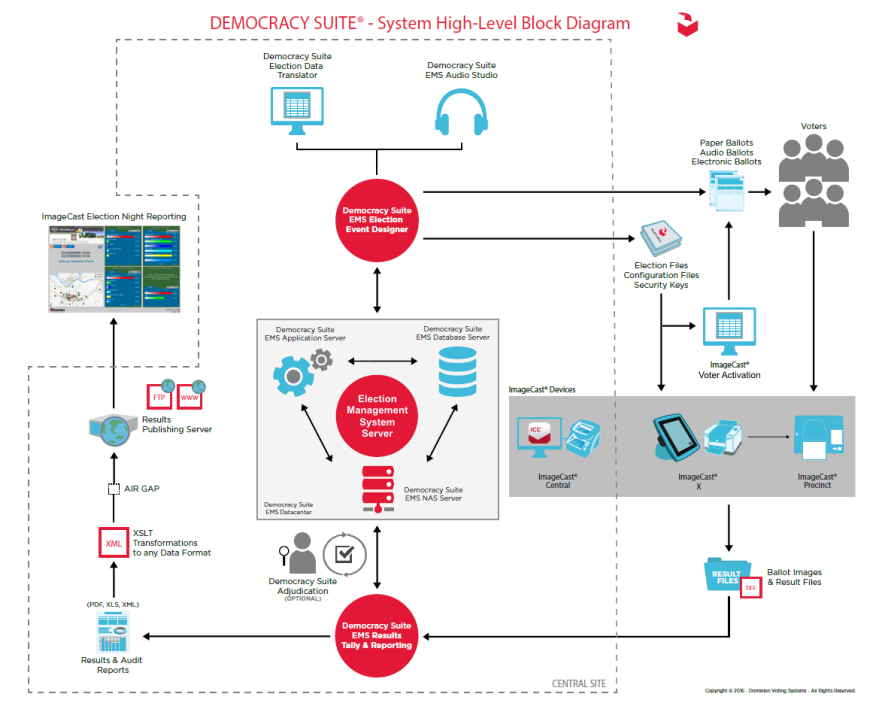
\includegraphics[width=\textwidth]{dominion.PNG}
    \caption{Block diagram of the native and virtualised Dominion voting scheme\cite{franklin2012interpreting}}
\end{figure}
\smallbreak \noindent
Specifically, allegations about data manipulation, miscounts, illegitimate votes and other oddities in the Dominion machines and systems to cast and count votes in numerous voting districts during the November election. While this work does not seek to engage with the veracity of these allegations, it seeks to produce a system with the security mechanisms and transparency that would either definitively prove these allegations, or definitively establish the integrity of this aspect of the election. This work will also develop a solution that is significantly more cost-effective, as the decentralization of blockchain allows for fair pricing, when compared to the federal 'carte blache' given to Dominion.\cite{murdockmulti}

\subsection{Project Proposal}
The proposal of the project is to utilize the growing technology known as blockchain, and its numerous strengths in terms of security and transparency, to supplant the current E-voting system which Dominion is a part of. The specifics of achieving this, will be delineated in the following sections of the report, after a brief discussion of what a blockchain is and offers.      

\section{Literature Review}

\subsection{Blockchain}
Blockchains are cryptographically secure,  distributed ledger which can hold records on any smart contract that is called on the blockchain. As the name entails, is a sequence of blocks linked cryptographically, usually by hashing the timestamp associated with each new data creating event.\cite{hawk1} These blocks each contain information on any supported smart contracts called on the chain, most commonly individual transactions and movements of the cryptocurrency they maintain. This is depicted in the figure below
\begin{figure}[ht!]
    \centering
    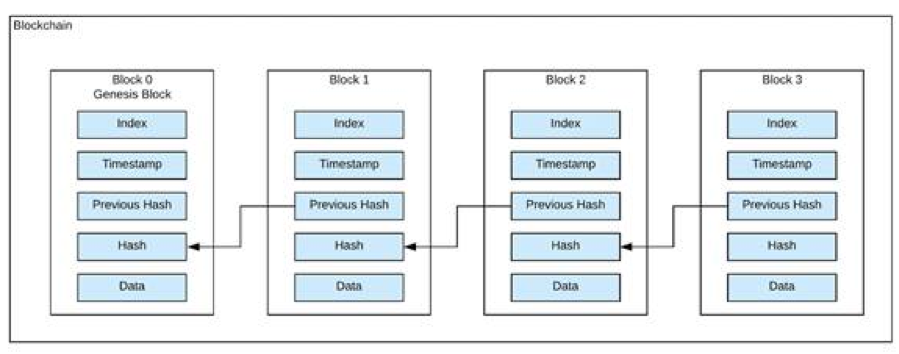
\includegraphics[width=0.75\textwidth]{blockchain.PNG}
    \caption{Applications supported on the NEO blockchain}
\end{figure}
\smallbreak \noindent
A blockchain often uses multiple separate servers which function as nodes. These nodes record, share, and synchronize the transactions in their respective electronic ledgers. This is what allows them to maintain their two strongest selling points, decentralization and security. A natural consequence which emerges from multiple devices across different networks verifying and checking against each other to ensure the blockchain has not been modified or tampered with by an outside entity.\cite{hawk1} This characteristic, alongside strong cryptographic protocols, make blockchains almost completely resistant to modification, which is inimical to ensuring the security and reliability of the ledger. 
\smallbreak
\noindent
As a result, the only known adverse event that could feasibly lead to the manipulation of a blockchain is a '51 percent attack' or '67 percent attack' depending on the validation algorithm run by the blockchain. This attack, as the name indicates is one where either half or two-thirds of all nodes/miners running on a blockchain were to be compromised and hash blocks with incorrect or manipulated data. Taking Bitcoin as an example, it has been shown that no single individual, entity, institution, or government possesses enough computing power to perform this sort of attack and overwrite the ledger. While Bitcoin is the blockchain with the most computing power at its disposal, most mature and adopted blockchains possess enough computing power that from  a risk assessment perspective, the probability of a successful attack is infinitesimally small. In addition to this, almost all blockchains have oracles and built in smart contracts to freeze or protect the blockchain should an attack be detected. 
\smallbreak
\noindent 
Users and programs can interact with a blockchain through a construct known as a smart contract.\cite{vox1} In the context of blockchains, smart contracts represent programs that delineate transaction protocols. Essentially, they are highly secure algorithms that control the distribution and ownership of a cryptocurrency. The network of nodes that maintain the blockchain verify that the smart contracts have not been tampered with.\cite{hawk1} A simple example of a smart contract process would be when a fee payment is made to the Ethereum blockchain. When a user completes a payment, a program sends the record of this transaction to a smart contract, which updates the blockchain to include this movement of funds and issues the corresponding Ethereum to the cryptocurrency wallet associated with the user. This transaction record is then synchronized with all the nodes in the blockchain.\cite{vox1}
\smallbreak \noindent
For the purposes of this project, we will explore those blockchains that support the following services:
\begin{itemize}
    \item In chain, third party tokens 
    \item Token distribution
    \item Token ownership
    \item Public block explorer and private address system.
    \item Non-fungible token attribution.
\end{itemize}
This will allow for a system to be created where voting tokens are given on a one-to-one basis for voters, and voters can cast their vote through the execution of a smart contract. Said smart contract will track data that will allow to verify the validity of a vote, while maintaining the anonymity of the voter. Alternatively, votes could be cast as a non-fungible token, once again ensuring that the owner of the token is a legitimate voter through calling a smart contract on the chain.
\smallbreak \noindent 
From the perspective of cost, all that would be needed is for the federal government enough gas currency(cryptocurrency required to run smart contracts on a blockchain) to perform the 10s of millions of votes on the chain. Considering that each dominion voting machine cost upwards of 100,000 dollars, the gas fees would almost certainly be cheaper. This will not be fully explored till later on in the development of the project.

\section{Open Source Research}
Fortunately, most blockchains, cryptocurrencies, and tokens are open source. So we truly do have our pick of the bunch when selecting a blockchain to build on.

\subsection{Bitcoin}
While the discussion on Bitcoin, will be brief,and ultimately dismiss the blockchain, its status as the most widely adopted and famous blockchain means its always worth mentioning. Bitcoin,in its current state only supports token ownership and distribution, nowhere near our established requirements for the blockchain voting system proposed. Additional, the cost of transaction and node confirmation/consolidation times are prohibitively long. That being said, Bitcoin and its creator are of tremendous importance in the creation of digital currencies and blockchains.\cite{budish2018economic}

\subsection{Ethereum}
Without a doubt, the Ethereum network and ERC-20 protocol is the most developed, robust, matured, and proven blockchain system out there. Also called the 'World Computer', Ethereum allows for on-chain third party tokens, token distribution, token ownership, public block explorer, non-fungible token attribution and private address system. Additionally, Ethereum allows for the outsourcing of computation, governance systems, complex oracles, test net experimentation and many other use cases. On the downsides, Ethereum's gas token, ETH, is notoriously expensive and block times are rather slow.\cite{di2020tokens}
\smallbreak\noindent
However, the Ethereum blockchain is expecting a massive upgrade dubbed ETH2.0, estimated to take place in 2024. This would theoretically resolve the issues with gas fees and block time.
\begin{figure}[ht!]
    \centering
    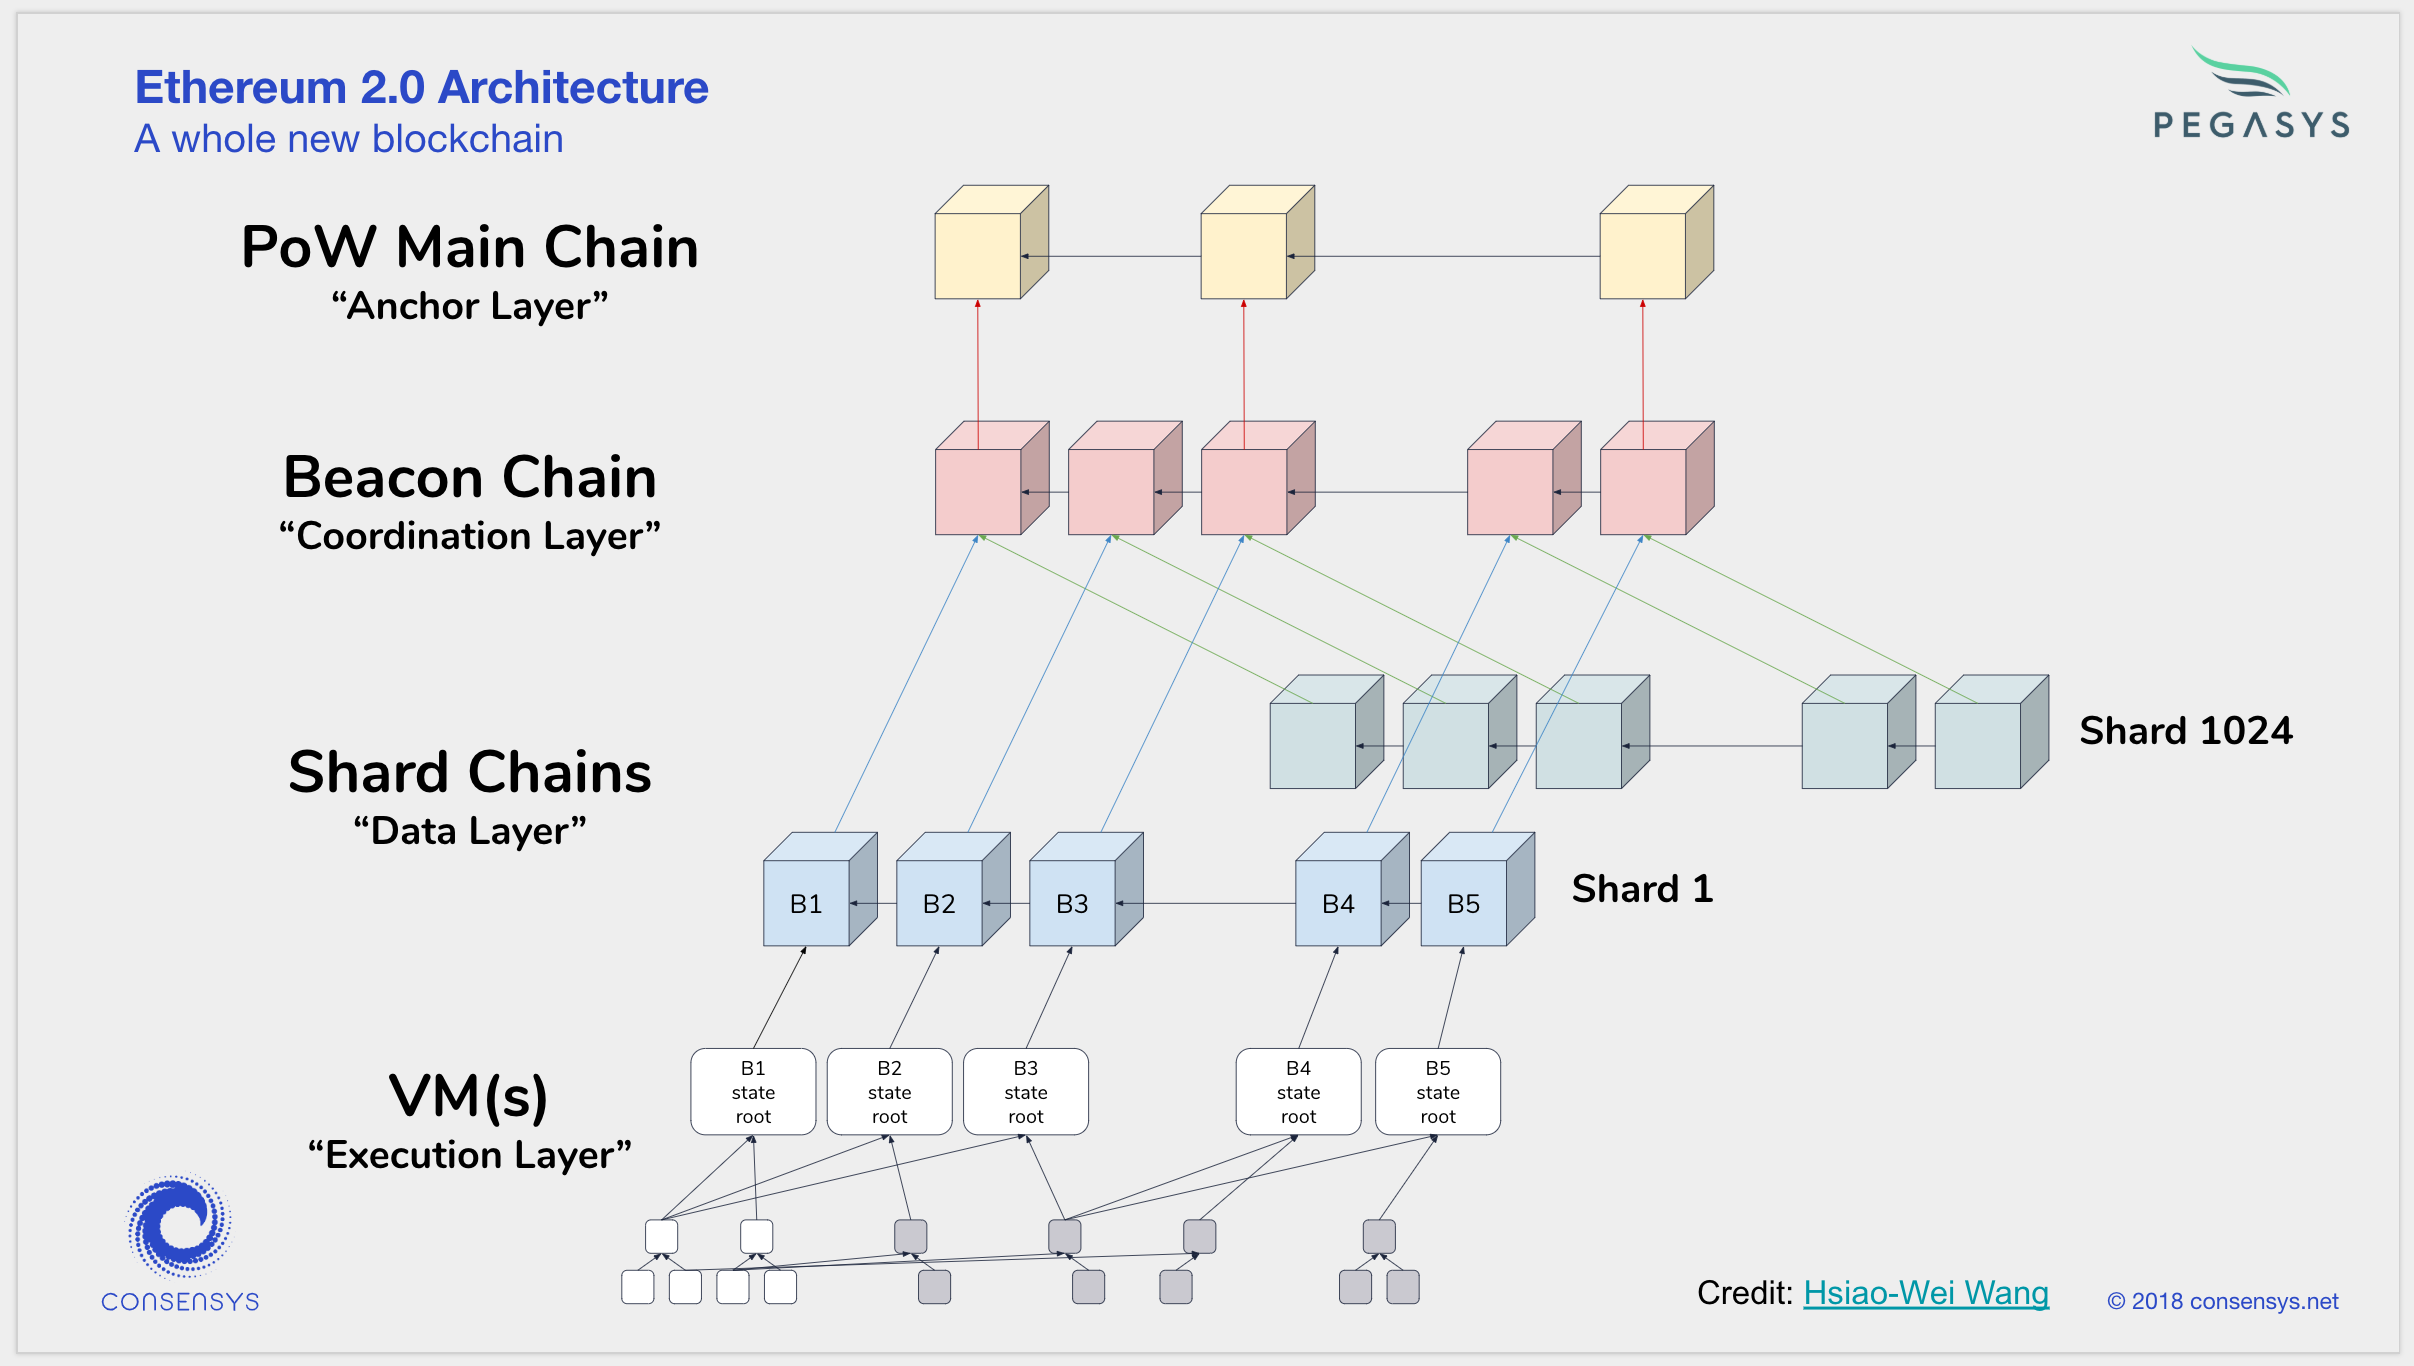
\includegraphics[width=\textwidth]{eth2.png}
    \caption{Proposed architecture of ETH 2.0}
\end{figure}

\subsection{NEO}
\smallbreak
NEO is not as developed as ethereum, but still contains the necessary services to develop the voting system. Additionally,its gas fees and block times are exceptional, and its block explorer API would be tremendously useful to create a voting transparency application.\cite{elrom2019neo}
\begin{figure}[ht!]
    \centering
    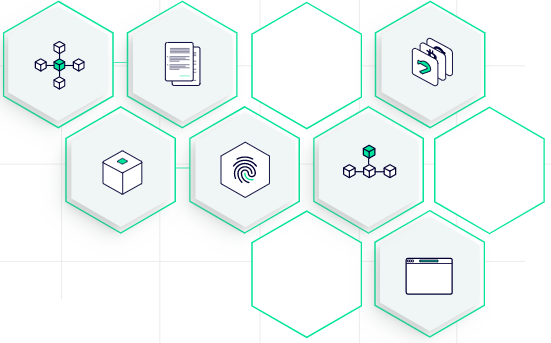
\includegraphics[width=0.6\textwidth]{neo_tech.PNG}
    \caption{Applications supported on the NEO blockchain}
\end{figure}

\subsection{Algorand}
Algorand only recently implemented a fork capable of NFT creation. Its block times and gas fees also makeit exceptional among the competition. \cite{gilad2017algorand}

\section{Duplicate the Results}
You can find, on the github repository, an example of NFT creation and deployment on a public Ethereum testnet.

\bibliographystyle{plain}
\bibliography{bibliography}
\end{document}